\section{初步研究}
本节我们对大模型的模型结构进行初步的介绍和分析,并从理论和实验两方面分析使用拆分学习进行大模型隐私推断时的严重隐私泄漏问题。

\subsection{大模型结构}
当前的大语言模型都是基于Transformer架构~\cite{vaswani_2017_attention}实现的,其模型可以分为3层,分别是:
\begin{enumerate}[label=(\arabic*)]
    \item 输入词向量(Word Embedding):即一个嵌入向量矩阵$E \in \mathbb R^{n\times d}$,其中$n$表示词汇表大小,$d$表示词向量的维度,一般为4096。
    %
    当输入$n$个单词(Token)后,其输出为$n \times d$大小的矩阵。
    %
    \item Transformer层:包含了多层Transformer结构,对隐层表征进行多次变换,其输入和输出的矩阵大小均为$n \times d$(此处忽略批样本情况,只考虑单个样本)。
    \item 输出词向量:与输入词向量相同,包含了一个矩阵$E' \in \mathbb R^{n\times d}$,且一般来说$E' = E$。
    当获得Transformer层的输出后,对输出的最后一行计算分数$\bvec  s = E'\bvec h$,表示输出单词的概率分布。
\end{enumerate}

其中Transformer层的关键模块是多头自注意力机制(Multi-Head Self-Attention,简称MHA)。
%
该模块会融合文本中不同位置单词(上下文)的信息产生输出,而其他模块仅仅对当前位置的表征进行变换。
%
具体而言,对于隐层表征$H \in \mathbb R^{n\times d}$,多头自注意力机制的运算包含如下步骤:
\begin{enumerate}[label=(\arabic*)]
    \item 产生查询(Query)、键(Key)、值(Value)对应的向量:对于任意一个位置的隐层表征$\bvec h \in H$,通过线性投影产生对应的$\bvec q = W_q \bvec h, \bvec k = W_k \bvec h, \bvec v = W_v \bvec h \in \mathbb R^d$。
    %
    \item 将所有的查询、键、值向量分割为维度为$d'$的子向量(注意力头),总共$d/d'$个,并对其进行位置嵌入(Positional Embedding)变换,一般而言是对向量逐元素地加或乘一个和当前单词所在位置相关的固定向量。
    %
    \item (对于每个注意力头)对于第$i$个查询$\bvec q_i'$,将其与当前存在的所有的键$\bvec k'_j$作内积得到分数$s'_{i, j} = \bvec q_i' \cdot \bvec k_j, j = 1\cdots n$。
    对这些分数进行Softmax归一化后再计算加权的值向量和 $\bvec h'_i = \dfrac{\exp {s'_{i, j}}}{\sum_{k = 1}^n \exp {s'_{i, k}}} \cdot \bvec v_j \in \mathbb R^{d'}$,这是当前的注意力头的输出。
    %
    \item 将各个注意力头的输出拼接起来,得到多头注意力的输出$\bvec h_i = \mathsf{concat}(\cdots, \bvec h'_i, \cdots)$。
\end{enumerate}

从上述分析中可以看出,注意力机制将不同位置(也就是不同输入单词)对应的表征进行了相互融合,从而捕捉文本中上下文的关系。
%
大语言模型在生成文本时,需要采用迭代生成的方式,即将前一轮的输出单词拼接到当前的输入语句中,然后再次输入模型预测下一个单词。
%
由于我们仅仅需要最后一个单词对应的表征,我们可以把之前MHA中计算出来的键向量和值向量缓存下来,从而只需要把最后一个单词输入模型中即可计算,从而避免重复计算。
%
这种技术被称为键值缓存(KV Cache)~\cite{pope_2023_efficiently_kv_cache}。
%
Transformer的其他模块包括全连接层(Fully-Connect Layer)、层归一化(Layer Normalization)模块,以及残差连接,是普通神经网络中的常用模块,在此不再赘述。
%
\autoref{fig:perm-llm_llm-arch}展现了一个典型的大语言模型的网络结构。

\begin{figure}[htbp]
    \centering
    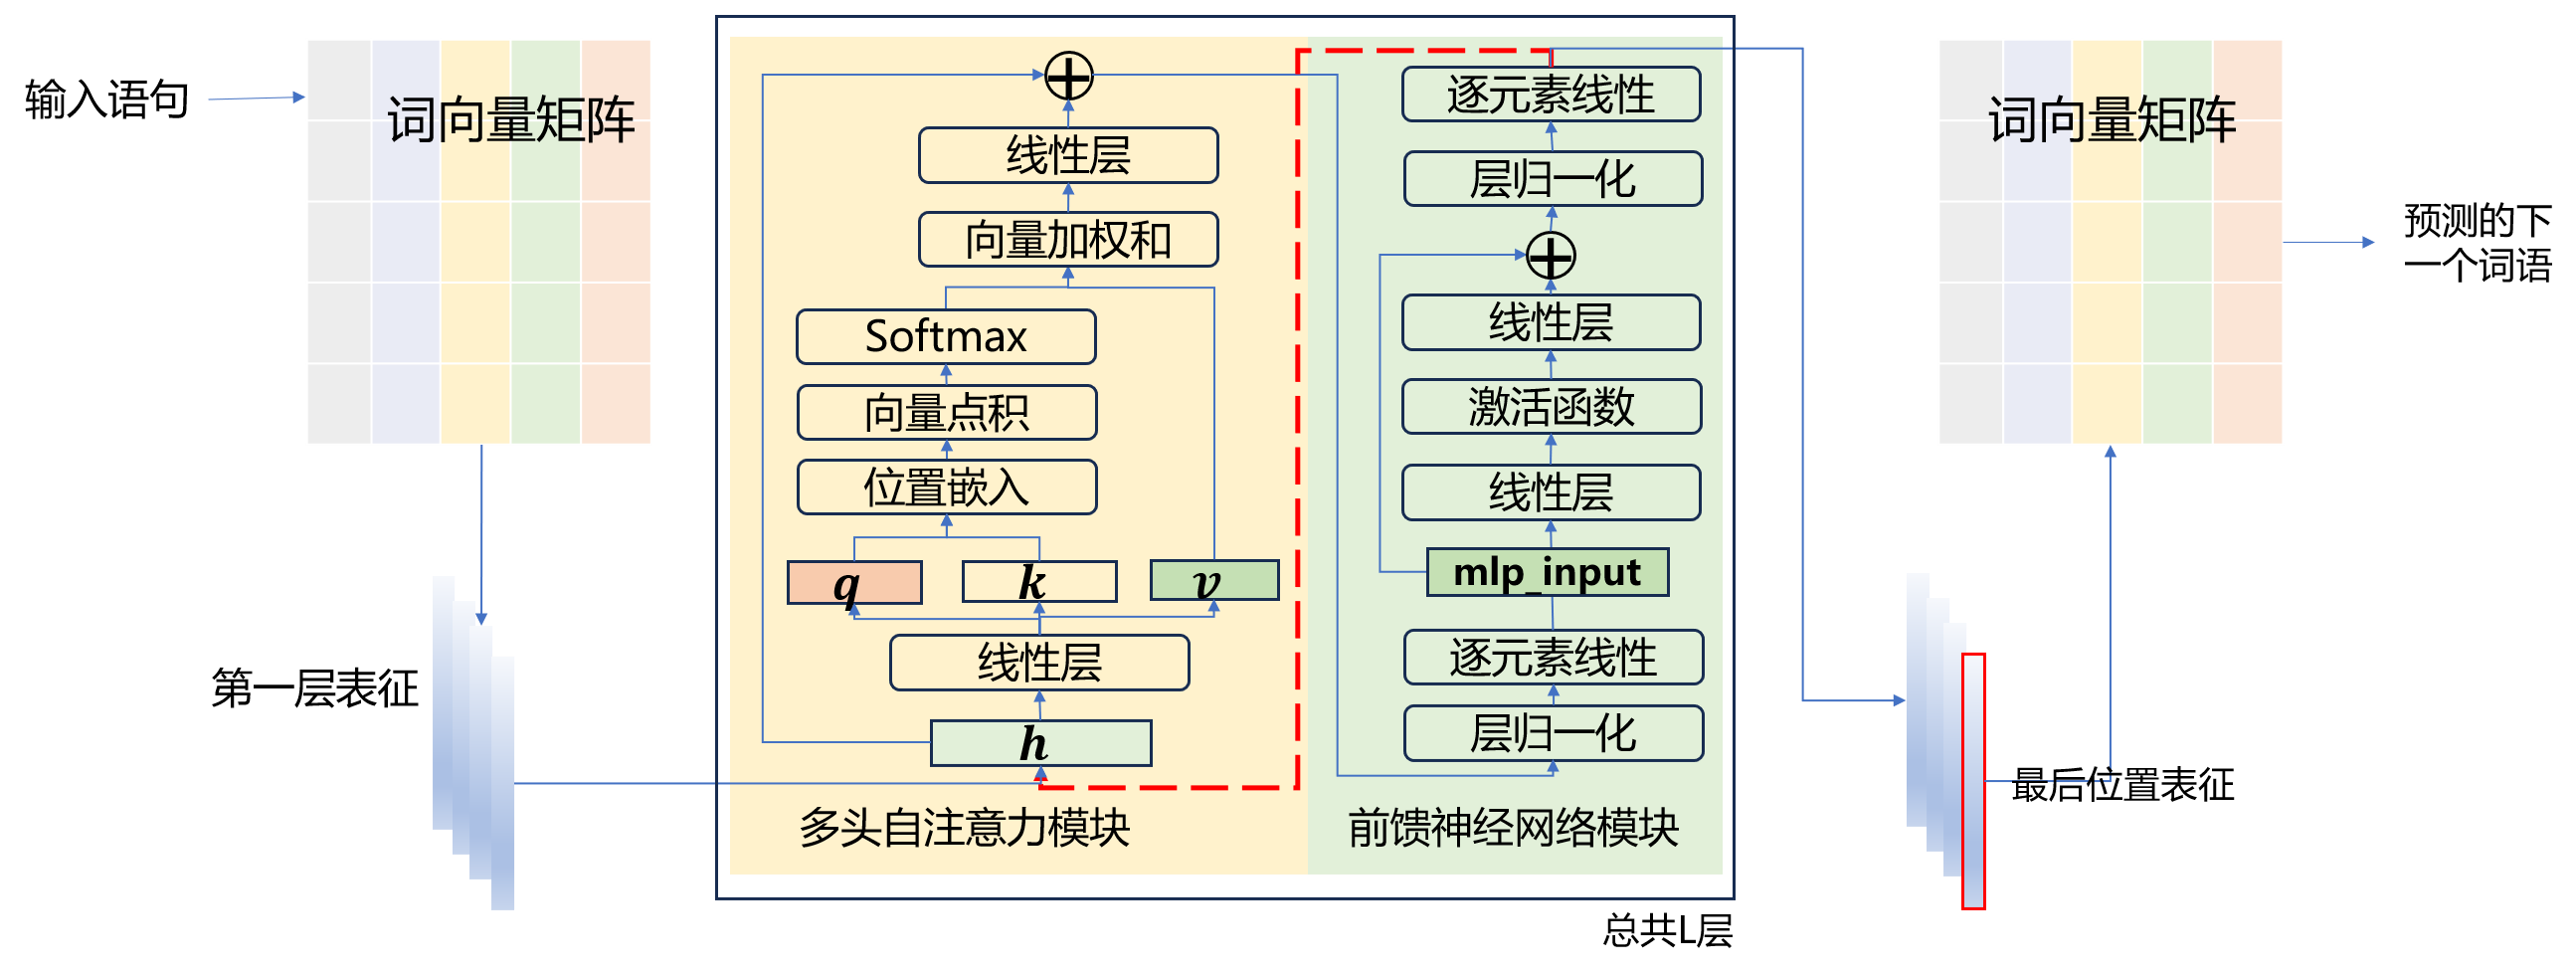
\includegraphics[width=\linewidth]{Z_Resources/perm-llm_llm-architecture.png}
    \caption{大语言模型结构示意图}
    \label{fig:perm-llm_llm-arch}
\end{figure}


\subsection{针对大模型拆分学习的攻击}
从上节的大模型结构描述中可以看出,大模型的隐层表征在每一层Transformer的变换中都保持着同样的大小,即$n \times d$($n$ 表示输入语句长度,$d$表示表征维度)。
%
因此从直观角度理解,大模型隐层表征包含了大量的输入信息。
且由于其隐层表征的尺寸随着层数增加保持不变,可以猜测即使是高层的隐层表征,依然包含着足够多的输入数据的信息。
%
已有研究提出可以通过训练逆向模型的方式从表征中恢复原始原本,无需知道模型的具体参数~\cite{morris2023embedding_almost}。
而本节则考虑攻击者已知模型参数的情况,更符合大模型的实际应用场景。


在拆分学习的大模型推断场景中,大模型被划分为一个底部模型$M_b$和一个顶部模型$M_h$。
%
我们假设模型拥有方最初拥有整个模型$(M_b, M_h)$,这也符合当前大模型训练是中心化的实际情况。
%
为了实现拆分学习的推断,模型拥有方将$M_b$发送给用户。
%
这种情况下,用户需要发送底部模型产生的表征$\bvec h = M_b(\bvec x)$给模型拥有方,其中$\bvec x$表示用户的输入文本对应的下标向量。

\subsubsection{表征逆向攻击}
当模型拥有方获取用户输入的表征后,就可以进行白盒攻击~\cite{hezecheng_2019_model_inversion_attack},通过如下的优化问题来猜测用户的输入:
\begin{equation}
    \label{eq:perm-llm_split-attack-0}
    \min \Vert M_b(\bvec x') - M_b(\bvec x)\Vert^2,
\end{equation}
其中$\bvec x'$是模型拥有方猜测的用户输入,$\bvec x$是用户的实际输入。
%
注意到直接对$\bvec x'$进行优化是较为困难的,因为其值域是离散的单词下标。
虽然可以转化成独热向量(One-Hot Vector),但是其依然具有离散的约束从而导致优化难以进行。
%
为此,模型拥有方可以首先优化初始表征$H'$,也就是词向量矩阵与(猜测的)用户输入对应的独热向量乘积:$H'_i = E\ \mathsf{onehot}(x'_i)$。
%
我们让$T_b$为底部模型除去词向量层(第一层)产生的模型,则我们可以把\autoref{eq:perm-llm_split-attack-0}改写为
\begin{equation}
    \label{eq:perm-llm_split-attack-1}
    \min \Vert T_b(H') - M_b(\bvec x)\Vert^2.
\end{equation}
由于此时优化变量$H'$属于连续变量,同时注意到$T_b$是模型拥有方已知的,因此我们可以直接用梯度下降等方法对\autoref{eq:perm-llm_split-attack-1}进行优化。
%
此时上述优化问题的未知数个数($H'$中的元素个数)与方程个数相等($M_b(\bvec x)$的元素个数),均为$nd$个元素,因为我们认为这个优化问题可能存在唯一的最优解,也就是$H' = H := (E\ \mathsf{onehot}(x_1), \cdots, E\ \mathsf{onehot}(x_n))$。
%
当得到猜测的表征$H'$之后,对于其中的第$i$行,使用余弦相似度计算出其最相似的词向量:
\begin{equation}
    \text{最相似单词下标} = \mathop{\text{argmax}}_i \dfrac{\bvec h'_i \cdot \bvec e_i}{\Vert \bvec h'_i \Vert\Vert \bvec e_i \Vert},
\end{equation}
其中$\bvec e_i$表示词向量矩阵的第$i$行。

综上所述,从大模型隐层表征恢复出用户输入文本的过程可以分为恢复第一层表征和从第一层表征恢复单词两步。
%
通过上述提出的两步方法,攻击者可以从隐层表征逆向推理出输入文本中每一个位置的单词,从而窃取用户的输入数据。
%

\subsubsection{可能的防御机制}
对数据加噪声是一种常用的隐私保护方法,并且在特定情况下可以达成差分隐私~\cite{dwork_2006_differential_privacy}。
%
因此,本节我们考虑在隐层表征中加入噪声进行防御的手段~\cite{morris2023embedding_almost}。
%
当用户算出底部模型产生的表征$H$后,对其进行扰动得到
\begin{equation}
    \tilde H_{ij} = H_{ij} + \lambda \cdot \epsilon, \quad \epsilon \sim \mathcal N(0, 1), 
\end{equation}
其中,$\lambda$表示噪声的大小。
%
越大的噪声一般可以实现越好的保护效果,但是也会产生更多的精度损失,损害模型性能。

\subsubsection{实验分析}
为了进一步测试上述攻击方案的可行性,我们在ChatGLM-6B模型~\cite{zeng_2022_glm130b}上进行了实验。
%
我们选用了Squad~\cite{2016_squad}和FindSum~\cite{2022_findsum}两个数据集进行实验,分别对应较短的文本和较长的文本。
%
对于每个实验,我们都对200个输入进行测试并且求其平均值。
%
攻击准确率的定义如下:
\begin{equation}
    \text{准确率} = \dfrac{1}{n} \sum_{i=1}^n \left( \dfrac{1}{l_i} \sum_{j=1}^{l_i} 1_{t'_{i,j} = t_{i,j}} \right),
\end{equation}
其中,$n = 200$表示总共的输入文本数,$l_i$表示第$i$个文本的长度,$t'_{i,j}$和$t_{i,j}$表示攻击得到的和实际的第$i$个文本的第$j$个单词。
%
由于ChatGLM-6B模型总共包含了28个Transformer层,我们设置拆分层分别为第10层和第20层。
%
我们使用梯度下降算法迭代优化\autoref{eq:perm-llm_split-attack-1}直到$H'$和$H$的余弦相似度达到0.98或迭代步数达到1000步为止。
%
我们使用半精度浮点数进行运算。

\begin{figure}[h!]
    \centering
    \begin{subfigure}{0.48\linewidth}
    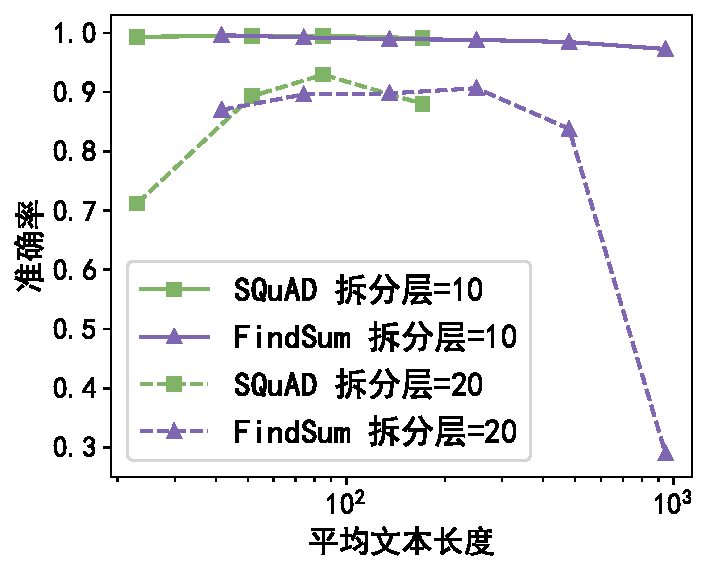
\includegraphics[width=\linewidth]{Z_Resources/perm-llm_seqlen-acc.pdf}
    \caption{攻击准确率}
    \end{subfigure}
    %
    \begin{subfigure}{0.48\linewidth}    
    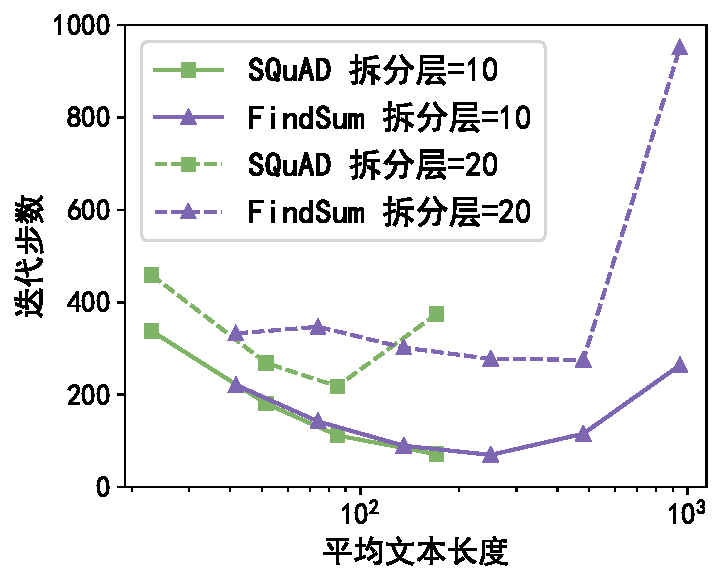
\includegraphics[width=\linewidth]{Z_Resources/perm-llm_seqlen-steps.pdf}
    \caption{攻击所需迭代步数}    
    \end{subfigure}
    \caption{攻击效果与文本长度的关系}
    \label{fig:perm-llm:attack-seqlen}
\end{figure}


\begin{figure}[h!]
    \centering
    \begin{subfigure}{0.48\linewidth}
    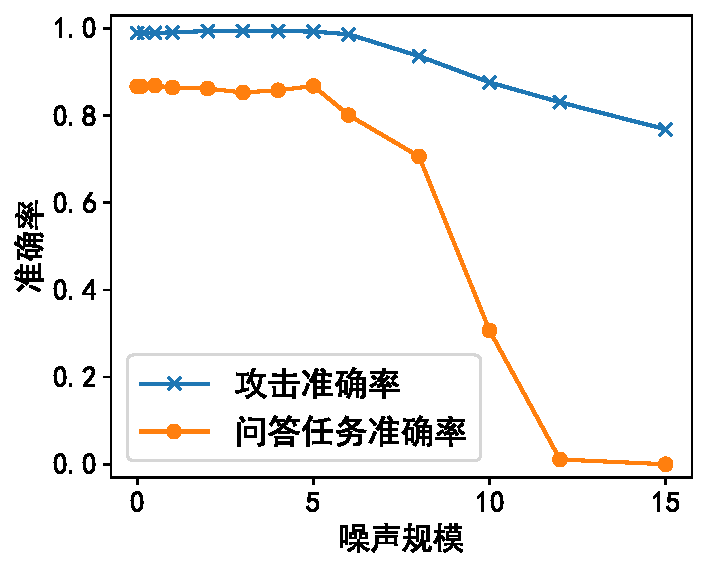
\includegraphics[width=\linewidth]{Z_Resources/perm-llm_squad-noise-layer10.pdf}
    \caption{拆分层=10}
    \end{subfigure}
    %
    \begin{subfigure}{0.48\linewidth}    
    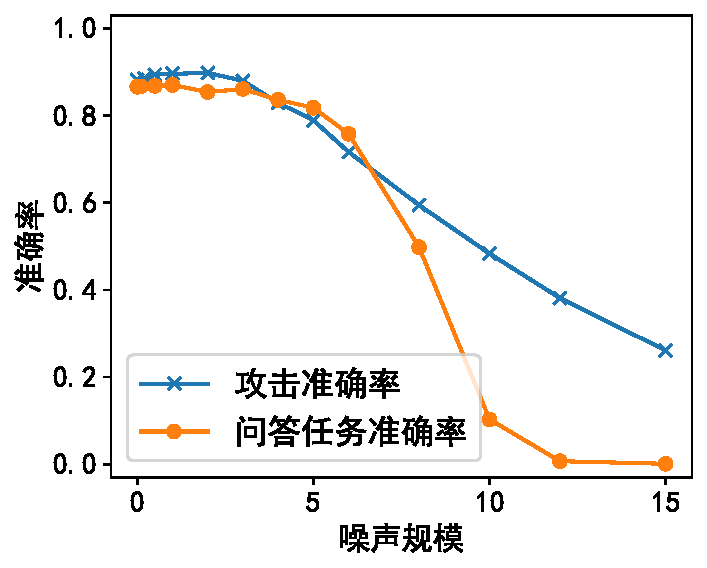
\includegraphics[width=\linewidth]{Z_Resources/perm-llm_squad-noise-layer20.pdf}
    \caption{拆分层=20}    
    \end{subfigure}
    \caption{攻击效果与噪声大小的关系}
    \label{fig:perm-llm:attack-noise}
\end{figure}

%
我们首先测试了对于不同输入语句长度的逆向攻击效果,测量了逆向攻击用户输入文本的准确率以及迭代所用次,并呈现在\autoref{fig:perm-llm:attack-seqlen}中。
%
从图中可以看出,在拆分层为第10层时,无论文本长度多长,攻击都能达到接近100\%的准确率;而拆分层在20层时,攻击准确率略有下降,大概为90\%左右。
同时我们注意到,文本长度特别长(1000左右)或特别短(个位数)时,攻击效果也会下降。
%
特别是文本长度达到1000时,攻击效果下降明显,但是此时迭代步数也达到了我们预设的最高值,因此可能在更多的迭代步数下会达到更高的效果。
%
此外,提高浮点运算的精度(比如从16位半精度提升到32位单精度)也可能会提升攻击效果。


我们也在Squad数据集上测试了噪声规模$\lambda$的大小对攻击效果以及原始任务效果的影响。
其中原始任务的准确率指的是问答任务的准确率,按照大模型返回的字符串中是否包含参考答案的字符串来计算,若包含则为回答正确,反之则为回答错误。
%
我们将结果汇报在\autoref{fig:perm-llm:attack-noise}中。
%
可以看到,随着噪声规模的增加,攻击准确率呈现出下降趋势。
然而原始的问答任务准确率也同步开始下降,并且下降速度更快,下降幅度更大。
%
在拆分层为第10层时,当问答任务的准确率已经变成0之后,攻击准确率依然有80\%以上。
在拆分层为第20层时,两者的下降幅度更加接近,但是问答任务准确率依然在$\lambda \ge 5$后下降得更快并且很快归零。
%



上述的实验分析表明,攻击者可以通过大模型拆分层的表征,有效地以很高精度还原出用户的原始输入。
%
对拆分层表征添加噪声的防御手段并不能有效地避免此种攻击,因为其会更严重地降低模型本身准确率。
%
这说明拆分学习不适用于大模型隐私推断的场景。
